\subsection{%
  Множества, отношения, операции%
}
\begin{example}[1]
\hangindent=4.9em
\hangafter=1
$A = \{\,-1,\hspace{1mm}\sqrt[]{2},\hspace{1mm}\pi\,\}$ --- перечисление\\[2mm]
$B = \{\, x \in \mathbb{R} \mid |x| \le 5 \,\}$ --- задано свойством\\[2mm]
$\mathbb{N} \subset \mathbb{Z} \subset \mathbb{Q} \subset \mathbb{R} \subset \mathbb{C}$ --- множество чисел\\[2mm]
$\emptyset$ --- пустое множество; $\{\,\emptyset\,\}$ --- одноэлементное множество
\end{example}
{\Large \textbf{!}} Множество не может быть своим элементом.
\begin{concept}[1]
Множество --- совокупность элементов, взятая как целое.
\end{concept}
\begin{concept}[2]
\underline{Отношение} (между множествами) --- соответствие, правило, сопоставление элементов множеств.
\end{concept}
\hspace{6em}%
\begin{tikzpicture}
    % Кружки маленького размера, пропорционально тексту
	\node[circle, draw, minimum size=1.5em, inner sep=1pt] (x) {$x$};
	\node[circle, draw, minimum size=1.5em, inner sep=1pt, right=2em of x] (y) {$y$};
	% Дуга со стрелкой и надписью
	\draw[->, bend left=40] (x.north) to node[below,font=\small] {$R$} (y.north);

	\node[right=1em of y, font=\small, align=left] (txt) {R --- Отношение};
\end{tikzpicture}\\[1mm]
\hangindent=6em
\hangafter=1
Запись:
\begin{tabular}[t]{@{}l@{}}
	$(\,x; y\,)$ или $x R y$ --- упорядоченная пара\\
	$\{\,x; y\,\}$ --- неупорядоченная пара $(x; y) \neq (y; x)$\\
\end{tabular}
\begin{definition}
	Отношение эквивалентности $(\, x \, \sim \, y\, )$ --- отношение,
	заданное свойствами (--- аксиоматические):
	\begin{enumerate}[topsep=5pt]
		\item \makebox[3cm][l] {$x \, \sim \, y$} --- рефлексивность
    	\item \makebox[3cm][l] {$y \, \sim \, x$ = $x \, \sim \, y$} --- симметричность
    	\item \makebox[3cm][l] {

		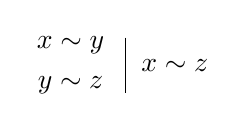
\begin{tikzpicture}[baseline=(current bounding box.center)]
			% Левая колонка
			\node (xy) at (0,1) {$x \sim y$};
			\node (yz) at (0,0.5) {$y \sim z$};

			% Вертикальная линия
			\draw (0.7,1.1) -- (0.7,0.4);

			% Справа по центру
			\node[right=0.5em] at (0.6,0.75) {$x \sim z$};
		\end{tikzpicture}} --- транзитивность
	\end{enumerate}
\end{definition}
\smallskip
\begin{figure}[h]
\centering
\begin{minipage}[t]{0.3\textwidth}
\begin{example}[1]
	\hangindent=5em
	\hangafter=1
	Равенство:\\[1mm]
	{$x \, = \, x$}\\
	{$x \, = \, y \implies y \, = \, x$}\\
	\hspace*{-0.3em}% Жесткий отступ
	\raisebox{-0.6\height}{% Центрируем по вертикали
	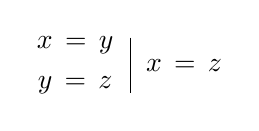
\begin{tikzpicture}[baseline=(current bounding box.center)]
		% Левая колонка
		\node (xy) at (0,1) {$x \, = \, y$};
		\node (yz) at (0,0.5) {$y \, = \, z$};

		% Вертикальная линия
		\draw (0.7,1.1) -- (0.7,0.4);

		% Справа по центру
		\node[right=0.5em] at (0.6,0.75) {$x \, = \, z$};
	\end{tikzpicture}}
\end{example}
\end{minipage}%
\hfill
\begin{minipage}[t]{0.7\textwidth}
\begin{example}[2]
	\hangindent=5em
	\hangafter=1
	Параллельность:\\[1mm]
	{$l \, \parallel \, l$}\\
	{$l \, \parallel \, a \implies a \, = \, l$}\\
	\hspace*{-0.3em}% Жесткий отступ
	\raisebox{-0.6\height}{% Центрируем по вертикали
	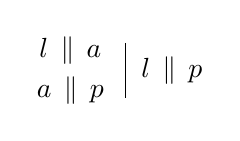
\begin{tikzpicture}[baseline=(current bounding box.center)]
		% Левая колонка
		\node (xy) at (0,1) {$l \, \parallel \, a$};
		\node (yz) at (0,0.5) {$a \, \parallel \, p$};

		% Вертикальная линия
		\draw (0.7,1.1) -- (0.7,0.4);

		% Справа по центру
		\node[right=0.5em] at (0.6,0.75) {$l \, \parallel \, p$};
	\end{tikzpicture}}
\end{example}
\end{minipage}
\end{figure}

\smallskip
\begin{concept}[1]
Алгебраическая операция --- набору элементов множества $M$ сопоставляется вполне определенный элемент множества $M$.
\end{concept}
\smallskip
\begin{example}[1]
	\stackunder{$a + b = c$}{\footnotesize (операция сложения)} \hspace{0.2em}
	$a, b, c \in \RR \larr{}$ бинарная операция\\
	\hspace*{19.8em} унарная ($\sqrt{a} = b$)
\end{example}
\smallskip
\begin{nota}
	Унарная, бинарная, триарная, $m$-арная - по числу элементов ($1, 2, 3,... m$)
\end{nota}
\begin{example}[1]
	$+, \times, \underline{\times \lambda \hspace{0.3em} (\lambda \in \RR)}$ --- унарная (элемент, умноженное на число)
\end{example}
